\documentclass{cubeamer}
\usepackage{ulem}
\usepackage{xcolor}

\title{Network Constraints on Species Coexistence ---or---}
\subtitle{the hubris of (a) man}
\author[Pat Wall]{Pat Wall}
\date{\today} % or whatever the date you are presenting in is
\institute[Indiana University]

\begin{document}

\maketitle

\cutoc

\section{Hubris}

\begin{frame}{Goals}
    \begin{columns}
        \begin{column}{0.7\textwidth}
            \begin{itemize}
                \item Build a useful Generalized Lotka-Volterra library in Rust
                \item Build a useful Microbial Genetic Algorithm library in Rust
                \item Evolve networks that allow high average species coexistence across random parameters using a combination of objective and novelty search
                \item Analyze resulting networks to find common structural features like directed cycles
                \item Simulate time series from simulated perturbation experiments and use transfer entropy to infer functional networks
                \item Compare structural and functional networks to see if we can find signatures of those structural features
            \end{itemize}
        \end{column}
        \begin{column}{0.3\textwidth}
            \begin{figure}
                \includegraphics[width=\textwidth]{assets/big-dog.png}
            \end{figure}
        \end{column}
    \end{columns}
\end{frame}

\begin{frame}{Outcomes}
    \begin{columns}
        \begin{column}{0.7\textwidth}
            \begin{itemize}
                \item Build a \sout{useful} Generalized Lotka-Volterra library in Rust
                \item Build a \sout{useful} Microbial Genetic Algorithm library in Rust
                \item Evolve networks that allow high average species coexistence using objective \sout{and novelty search}
                \item \textcolor{red}{\sout{Analyze resulting networks to find common structural features}}
                \item \textcolor{red}{\sout{Simulate time series from simulated perturbation experiments and use transfer entropy to infer functional networks}}
                \item \textcolor{red}{\sout{Compare structural and functional networks to see if we can find signatures of those structural features}}
            \end{itemize}
        \end{column}
        \begin{column}{0.3\textwidth}
            \begin{figure}
                \includegraphics[width=\textwidth]{assets/little-dog.png}
            \end{figure}
        \end{column}
    \end{columns}
\end{frame}

\section{Background}

\begin{frame}{The Paradox of the Plankton --- Hutchinson 1961 [cite]}
    \begin{figure}
        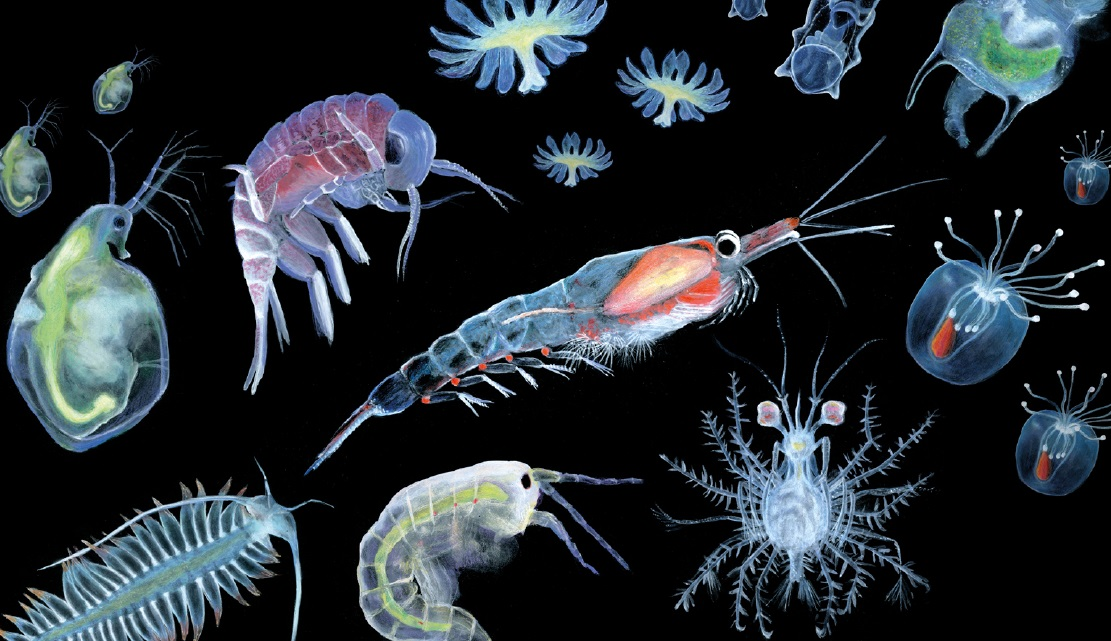
\includegraphics[width=0.9\textwidth]{assets/real-plankton.jpeg}
    \end{figure}
\end{frame}

\begin{frame}{The Paradox of the Plankton --- Hutchinson 1961}
    \begin{figure}
        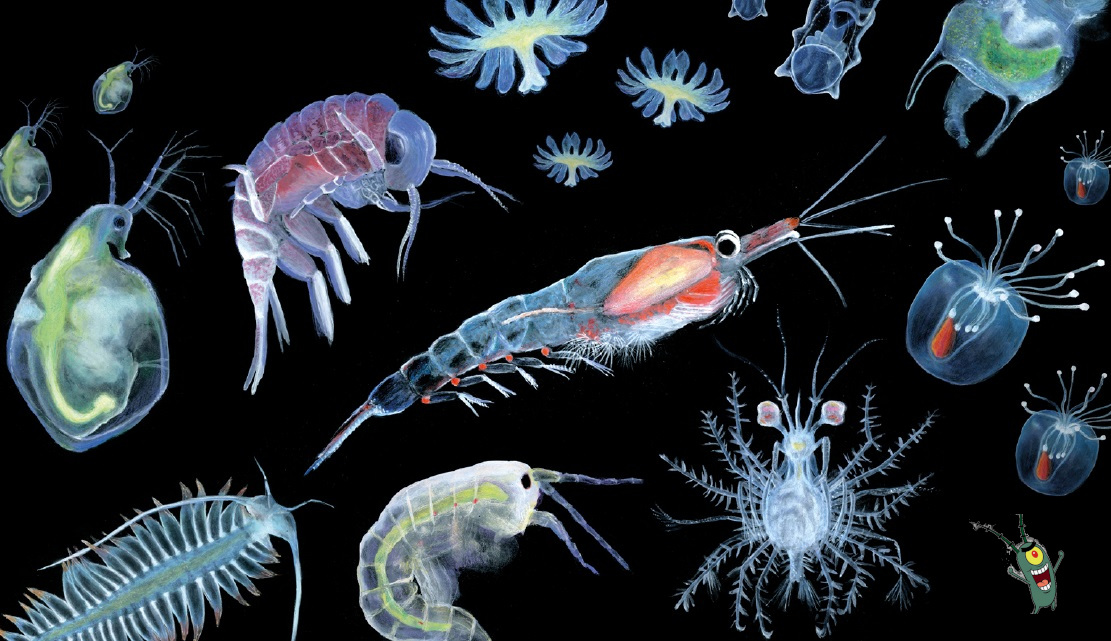
\includegraphics[width=0.75\textwidth]{assets/real-plankton1.jpeg}
    \end{figure}
    \begin{center}
        How can species coexist while competing for limited resources?
    \end{center}
\end{frame}

\begin{frame}{Resolutions to the Paradox}
    \begin{columns}
        \begin{column}{0.5\textwidth}
            \begin{enumerate}
                \item Niche Partitioning:
                \begin{itemize}
                    \item Differences in requirements \textit{and} impacts
                    \item Species stay out of each other's way
                    \item Tilman 1982
                \end{itemize}
                \item Storage Effect:
                \begin{itemize}
                    \item Mechanism to attenuate competitive effort
                    \item Species Opt-out of competition in bad times
                    \item Chesson 1994
                \end{itemize}
            \end{enumerate}
        \end{column}
        \begin{column}{0.5\textwidth}
            \begin{figure}
                \includegraphics[width=0.95\textwidth]{assets/letten_niche.png}
            \end{figure}
        \end{column}
    \end{columns}
\end{frame}

\begin{frame}{Nontransitive competition --- May and Leonard 1975}
    \begin{columns}
        \begin{column}{0.48\textwidth}
            \begin{itemize}
                \item Species all keep one another in check
            \end{itemize}
        \end{column}
    \end{columns}
\end{frame}

\begin{frame}{Transfer Entropy}
    \huge
    \begin{align*}
       T^{(k, l)}_{X \rightarrow Y}(t) &= I \left(X_t : Y_{t-1}^{l} \mid X_{t-1}^{k} \right ) \\
                                    &= H \left ( X_{t} \mid X_{t-1}^{k} \right ) - H \left ( X_t \mid    X_{t-1}^{k}, Y_{t-1}^{l} \right )
    \end{align*}
\end{frame}

\begin{frame}{Unpacking Transfer Entropy}
    \begin{columns}
        \begin{column}{0.7\textwidth}
            \begin{itemize}
                \item $k$: Target history length (ideally $k \rightarrow \infty$)
                \item $l$: Source history length (less clear)
                \item $Y_{t-1}^l$: Vector of historical states of Y with indices $(t-l, t-l+1, ..., t - 1)$
                \item $X_{t-1}^k$: Vector of historical states of X with indices $(t-k, t-k+1,..., t-1)$
            \end{itemize}
            
        \end{column}
        \begin{column}{0.3\textwidth}
            \begin{align*}
                T^{(k, l)}_{X \rightarrow Y}(t) &= I \left(X_t : Y_{t-1}^{l} \mid X_{t-1}^{k} \right )
            \end{align*}
        \end{column}
    \end{columns}
            
\end{frame}

\section{Estimation of Transfer Entropy}

\begin{frame}{What do we need to compute transfer entropy?}
\centering
  Transfer entropy is hard because we need lots of conditional distributions:
    
    Let's say that we have $k=5$ and 3 possible states $\{A, B, C\}$ for our source variable $Y$. In order to compute $T_{Y \rightarrow X}$ we need:
    
    \begin{enumerate}
        \item $p(X \mid A, A, A, A, A)$
        \item $p(X \mid A, A, A, A, B)$
        \item $p(X \mid A, A, A, B, A)$
    \end{enumerate}
    
    And so on, in this case its $3^5$ conditional distributions!!
\end{frame}

\begin{frame}{Bin Discretization}
\centering
    How can we estimate discrete PDFs from our data? In the simplest case:
    
    \textit{Bin discretization}
    
    \vspace{15}
    \begin{columns}
        \begin{column}{0.5\textwidth}
            Pros:
            \begin{itemize}
                \item Really easy!
                \item We've already seen it!
            \end{itemize}
        \end{column}
        \begin{column}{0.5\textwidth}
            Cons:
            \begin{itemize}
                \item Almost always biased
                \item Workaround quickly get more complex (e.g. adaptive bins)
            \end{itemize}
        \end{column}
    \end{columns}
\end{frame}

\begin{frame}{Fancy Estimators}
    In practice we use fancy estimators developed by computer scientists.
    
    Current state of the art is the Kraskov (KSG) estimator available in multiple open source packages including the Java Information Dynamics Toolkit (JIDT) that I use.
\end{frame}

\section{Applications of Transfer Entropy}

\begin{frame}{Vicsek Model}
    \begin{columns}
        \begin{column}{0.5\textwidth}
            img here
        \end{column}
        \begin{column}{0.5\textwidth}
            img here
        \end{column}
    \end{columns}
\end{frame}

\begin{frame}{Transfer Entropy in Vicsek Model}
\end{frame}

\begin{frame}{Transfer Entropy in Phase Transitions}
    img here
\end{frame}
    

% Q&A
\begin{frame}[standout]
    \centering
    \Huge\textbf{Thank You}
    
    \vfill
    
    \LARGE\textbf{Questions?}
\end{frame}
\end{document}
